
\section{Desarrollo}

Después de haber realizado el análisis inicial de el alcance del proyecto y las necesidades de los usuarios, se comenzó con el desarrollo del proyecto. Este desarrollo se hizo en tres partes. Primero, el desarrollo de un módulo de monitoreo de las estaciones meteorológicas por medio de drivers,  después un API como intermediaria entre la información almacenada en la base de datos y una interfaz gráfica para el monitoreo eficaz.

\subsection{Del módulo de monitoreo de estaciones}

El módulo de monitoreo de estaciones meteorológicas tiene como objetivo el observar la información obtenida por los diversos drivers de conexión a las estaciones meteorológicas y generar reportes conforme sea necesario, la lógica de reporte es tal como se muestra en la figura \ref{fig:logica_de_reporte}.

%! Agregar acciones al diagrama
%! Cambiar por diagrama de secuencia
% Agregar un fin después de generar la alerta
% debe hber un solo inicio y final

\begin{figure}[!ht]
	\centering
	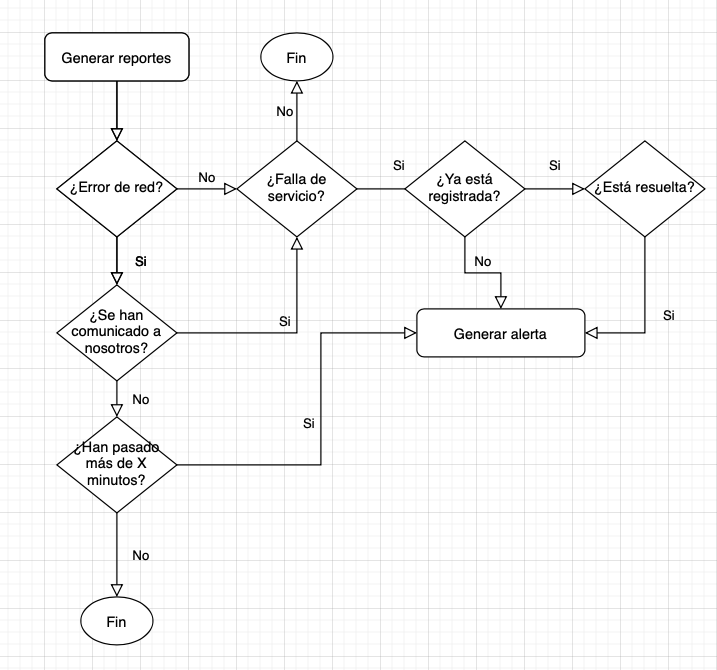
\includegraphics[width=1\linewidth]{images/diagrams/report_logic.png}
	\caption{Lógica de reporte del estado de las estaciones meteorológicas}
	\label{fig:logica_de_reporte}
\end{figure}


\subsection{Del API para el acceso a la información}

\subsection{De la interfaz gráfica del proyecto}

PAra el desarrollo del proyecto, se utilizó tailwind.

\section{Avances}


\section{Módulo de monitoreo}

\subsection*{Requisitos}

\subsection*{Seguridad}

\subsection*{Método de conexion}



\section{Selección de base de datos}

%! Terminar para la próxima

% Casi todas las secciones de desrrollo, van ligadas a una de resultados.

%? Escribir el proceso que realicé. Presentar lo suficiente para darle una idea al lector.

%? Presentar un fragmento de código más relevante. Incluir enlace a repositorio. La funcionalidad se puede expresar en algún tipo de representación gráfica.

%? Evitar párrafos de una sola oración. (Dar MÁS contexto), extranjerismos en itálica.
Con un tiempo de respuesta de $~[N]ms$, el sistema puede soprotar hasta N estaciones concurrentes.

Debido a que la recolección de los datos es por métodología pull y no push, es posible tener las estaciones en una cola que se ejecute hasta por un periodo de 5 minutos (que es un estándar en la recolección de datos de estaciones meteorológicas). Esto implica que la base de datos [X] puede soportar hasta [N x 60 x 5] datos de forma concurrente.

Tomando en cuenta las necesidades actuales del LCCA, y el estimado del tamaño de las redes de alta densidad (que pueden llegar hasta los N nodos como X artículo lo demuestra), no vale la pena el introducir la complejidad extra de un motor de base de datos desconocido y para el que no existen ORM's con soporte completo en el lenguaje de desarrollo. Porque no es un sistema de alta densidad de datos.

Si bien es posible escalar horizontalmente la infraestructura, se busca evitarlo ya que los \textit{diminishing returns} del costo de tener que mantener un sistema de monitoreo no es costeable. Para los casos de sistemas de extremadamente alta densidad, se recomienda el crear varias instancias seccionadas en bases de datos, o escalar la base de con un redis en vez de escalar.

%! Recordar que la información debe ser consultada desde el API, así que no sólo se tienen que tomar en cuenta la cantidad de query's por segundo que se requieren hacer para las inserciones, sino también para la consulta de datos.

%! Si lo que queremos es proveer herramientas para la gestión de calidad de los datos meteorológicos, la información tiene que tener en mente los principios Solidos y transaccionales, al menos en la creación de reportes basados en incidentes.
